\documentclass[a4paper, 10pt, openany]{book}%标注了文档类型和字号大小
\usepackage{geometry}

\geometry{left=3cm,right=3cm,top=3cm,bottom=3cm}
\usepackage[T1]{fontenc}
\usepackage{titlesec}
\usepackage{hyperref}
\usepackage{url} % 用于更好地格式化URL

\titleformat{\section}[block]{\normalfont}{\thesection}{1em}{}
\titleformat{\subsection}[block]{\normalfont}{\thesubsection}{1em}{}
\titleformat{\chapter}[display]
  {\normalfont\huge} % 设置章节标题的字体为正常字体(非加粗)
  {Chapter \thechapter}{1em}{} % 保留 "Chapter" 和 章节编号

\usepackage{xeCJK}
\usepackage{footmisc}
\usepackage[UTF8]{ctex}
\usepackage{amsmath}
\usepackage{subfigure}
\usepackage[graphicx]{realboxes}



\setCJKmainfont{FangSong}%中文设置为仿宋

\setmainfont{Palatino Linotype}%英文设置为palatino linotype

\begin{document}
  \title{ \heiti 平衡态统计物理笔记}
  \author{亦可}
  \maketitle
  \tableofcontents


  \newpage

  \chapter{写在前面/Foreword}
  \chapter{热学回顾/Thermodynamics}

  热学理论是唯象的,唯象的观点没有所谓对体系微观细节的认知,热力学定律基本来自实验和日常规律的总结。

  统计物理和热力学研究的核心问题,总是假定体系处于平衡状态。它们没有办法回答“如何达到平衡态”的问题。

\section{热平衡状态与第零定律}

\subsection{第零定律}
一般当我们提及平衡状态,我们指称的是,一个体系的某些性质随着观察的时间的推移不发生变化。

这是一个很值得推敲的说法。什么样的性质不随时间变化?如果我们试想一箱子气体,随着时间的推移,我们持续跟踪箱子中一个确定的粒子的性质,该粒子的动量(或者位置)当然是随时变化的,即使整个系统已经达到了所谓平衡。也就是说,热力学意义上的平衡是动态的。因此,我们所谓的不随时间变化,实际上已经隐含了宏观测量的描述:

\begin{itemize}
\item 测量的特征时间要比微观的运动时间长的多。

\item 我们测量的物理量一定是粗略的,缓慢的。
\end{itemize}

对于一个宏观系统,其自由度当然是很多很多的,要完整地、详尽地描述它需要极多的自由度。因此在我们所谓意义上的测量时,我们是提取了体系的一个特征来进行测量,即将一个超高维的相空间简化为了一些简单的热力学变量来进行测量。这些热力学变量需要符合前述“缓慢的、粗略的”定义。

有些热力学变量很直观,例如压强(描述了气体的力学特征),体积(描述了气体的几何特征)等。但这些特征并非热力学体系独有。那么,什么变量是跟“热”相关的特征量呢?我们当然已经知道这就是温度。

\vspace{10pt}

{第零定律:考虑三个系统A,B与C。A与C热平衡,且B与C热平衡,则可以推出A与B热平衡。}

\vspace{10pt}

\subsection{温度与物态方程}

第零定律如何说明了温度的存在?(注意,我们并没有要求ABC三个系统的相态。不过为了简单进行说明,我们可以考虑三个系统均为气体的情况。)


A与C热平衡,说明存在一个函数$f_{ac}$,满足方程(2.1)。
\begin{equation}
f_{AC}(p_A,V_A,p_C,V_C)=0
\end{equation}

同理,B与C热平衡,说明存在:
\begin{equation}
f_{BC}(p_B,V_B,p_C,V_C)=0
\end{equation}

改写一下,可以写为(2.3)的形式.
\begin{equation}
V_C=F_{AC}(p_A,V_A,p_C)=F_{BC}(p_B,V_B,p_C)
\end{equation}

第零定律表明,如果有上式成立,则应该有:
\begin{equation}
  f_{AB}(p_A,V_A,p_B,V_B)=0
  \end{equation}

即上推下。因此(2.3)式必可以约去$p_C$,因此有:
\begin{equation}
  g_1(p_A,V_A)=g_2(p_B,V_B)
  \end{equation}

  此时$g$既是温度函数,也是物态方程。
\begin{itemize}

\item eg1.理想气体的物态方程:$pV=Nk_BT$,其中$N$为粒子数。

\item eg2.范德瓦尔斯气体的物态方程:
\begin{equation}\begin{cases}(p+\frac{a}{v^2})(v-b)=k_BT \\ v=\frac{V}{N}\end{cases}\end{equation}

\end{itemize}

把理想气体\footnote{关于理想气体。}作为测温物质(因为其状态方程简单)(即C系统),可以定义温标。

\begin{equation}T=273.16K\frac{(pV)_{input}}{(pV)_{triple}}\end{equation}

其中$K$表示开尔文,是温度的单位。
\section{第一定律}

\subsection{第一定律的各种表述}
在探讨第一定律之前,我们需要先讨论几个有关对于“器壁”概念的描述并明确它们的定义。
\begin{itemize}
  \item “绝热”-系统与系统之间没有热交换。
 \item  “透热”-系统之间存在热交换。
 \item “孤立”-外界不能对系统做任何事。

\end{itemize}

\vspace{10pt}

第一定律:一个绝热的系统(改变状态的方式只有做功),从不同的做功路径,使系统从同初态到同末态,需要的功相同。

\vspace{10pt}

第一定律说明存在内能这个物理量(因为稳定的做功说明存在稳定的能量差),内能的定义通过式(2.8)完成。
\begin{equation}
W=U(p_2,V_2)-U(p_1,V_1)
\end{equation}

如果器壁变成透热的,则上式不成立。差距来自通过器壁的热交换,于是我们定义热量交换

\begin{equation}
  Q=U_2-U_1-W
  \end{equation}

更普遍更量化的第一定律就可以表示为下面的式(2.10):
\begin{equation}\Delta U=W+Q\end{equation}

也有很多时候,我们希望对过程进行细分化,这时候,我们需要用到第一定律的无穷小形式(2.11)
请注意这里$\text{\dj}$符号的使用,这表示该量与路径相关。


\begin{equation}\mathrm{d}U=\text{\dj}W+\text{\dj}Q\end{equation}

我们希望给$\text{\dj}W$和$\text{\dj}Q$一个用系统参量表示的表达式。出于这个目的,我们来讨论关于$W$的过程量的表达式,为此,我们需要引入准静态过程的概念。

准静态过程,指的是一个过程slow enough以至于在系统变化的任意时刻始终保持平衡状态。
在准静态过程下,做功的表达式如式:

\begin{equation}\text{\dj}W=-p\mathrm{d}v\end{equation}

更一般的情况下,有

\begin{equation}\text{\dj}W=\sum_{i}\textbf{F}_i\cdot \mathrm{d}\textbf{x}_i\end{equation}

其中,$\textbf{F}$是强度量,$\textbf{x}$为广延量(随体系的尺寸改变而改变)。


\subsection{热容}

定义热容:体系升高1开尔文所需要的热量。

\begin{equation}C=\frac{\text{\dj}Q}{\mathrm{d}T}\end{equation}

这里有两点值得注意。第一,热容是一个实验可测的量,许多物理问题都源于此。第二,该表达式中,吸热是依赖过程的量,所以热容也是依赖过程的。常用的热容有$C_v$和$C_p$分别为定容热容和定压热容。

\begin{equation}C_v=\left(\frac{\partial U}{\partial T}\right)_v\end{equation}

\begin{equation}C_p=\left(\frac{\mathrm{d}U+p\mathrm{d}V}{\mathrm{d}T}\right)_p=\left(\frac{\partial U}{\partial T}\right)_p+p\left(\frac{\partial V}{\partial T}\right)_p\end{equation}

这里,我们可以定义$H=U+PV$,此时$C_p$可以表示为:

\begin{equation}
C_p=\left(\frac{\partial H}{\partial T}\right)_p
\end{equation}

理想气体的绝热自由膨胀:该实验的结果表明,膨胀后的气体体积和压强都发生了变化,但是温度却没有变化,这说明理想气体的内能是温度的一元函数。可以得到
\begin{equation}U_{ig}=U_{ig}(T)\end{equation}


因此对于理想气体,有式(2.18)成立。

\begin{equation}C_p-C_v=p\left(\frac{\partial V}{\partial T}\right)_p=Nk_B\end{equation}

\section{第二定律}

\subsection{热机 }
对第二定律的探索来源于热机。围绕热机效率的研究催生了第二定律的表述。一般的,热机由高温热源+热机主体(向外做功)+向低温处放热的一整套循环系统组成。注意,高温热源并不一定要具有特定温度。循环中所有吸热的点都被认为处在高温热源。

且,尤其需要注意的一点是,由于是准静态过程,因此在吸放热时,系统的温度与热源或散热区一定要保持相同。\footnote{这里,我们需要重申一下可逆过程和准静态过程的关。一个没有耗散的准静态过程就是可逆过程。可逆过程一定是准静态过程。}

热机的主要功能是吸收热源的热量,并对外做功,当然,过程中热机还会放出一部分热量。对于此,我们总是希望热机尽可能多地把吸热转化为做功。也就是,如果我们定义热机效率:

\begin{equation}
  \eta =\frac{W}{Q_{in}}
\end{equation}

我们总是希望热机效率尽可能地高。显然,由于第一定律,我们知道:

\begin{equation}
\eta\leq1
\end{equation}

考虑热机的逆过程(不是很严谨,严谨地说只有可逆热机才有逆过程,不过你可以定性地想一想),我们可以构建制冷机,它的工作原理是:从低温热源吸热$Q_{in}$,同时受到外界做功$W$,最终对高温热源放出$-Q_{out}=Q_{in}+W$的热量。对于这种机器,我们关心的是制冷效果和做功之间的比例,因此我们定义制冷系数:
\begin{equation}
  \eta=\frac{Q_{in}}{W}\end{equation}

经过大量的实验观察,热力学第二定律终于得到总结。在经典的教材中,第二定律的克劳修斯表述和开尔文表述总是被给出。它们分别是:

\begin{itemize}
\item 克劳修斯表述:不可能将热从低温物体传递至高温物体,而不引起任何其他变化。

\item 开尔文表述:不可能存在这样一个热机,它从单一热源吸热,并把吸收的热量完全转化为做功。
\end{itemize}

克劳修斯表述和开尔文表述是等价的。要证明这组等价性,我们只需要证明,如果克劳修斯表述不成立,则开尔文表述也不成立;如果开尔文表述不成立,则克劳修斯表述也不成立。

\begin{itemize}
  \item 如果存在这样一种过程,除了热量从低温处传递至高温处,没有任何其它影响。我们就构建如图[2.1]的一个热机。在这个循环中,左侧是一个“克劳修斯热机”,它在单次循环中将$Q$的热量从低温热源传递至高温热源;右侧是一个正常的热机,它在单次循环中从高温热源吸热$Q_{H}$,做功$W$,并对低温处放热$-Q$,两者合并的效应就形成了一个“开尔文热机”,即完全从单一热源吸热并完全转化为功。即证明,如果克劳修斯表述成立,则开尔文表述同样不成立。
  
  \begin{figure}[h]
    \centering 
    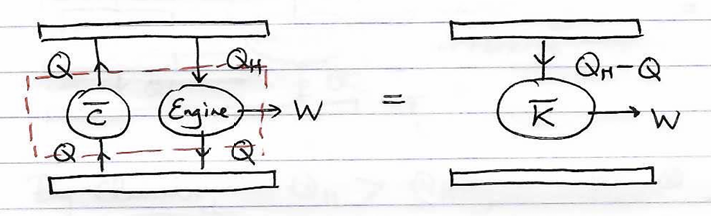
\includegraphics[height=4.0cm]{3.png}
    
    \caption{come from ZCYang}
    
    
    \end{figure}
  
  \item 如果存在这样一个热机,可以把吸收的热量完全地转化为功,那么,我们就可以设计如图[2.2]的一个系统。左侧是一个开尔文热机,类似地,整体就是一个克劳修斯热机。


  \begin{figure}[h]
    \centering 
    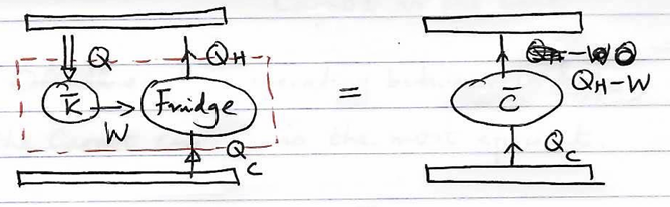
\includegraphics[height=4.0cm]{4.png}
    
    \caption{come from ZCYang}
    
    
    \end{figure}

\end{itemize}
\subsection{卡诺定理与热力学温标}
让我们继续热机的话题。对于此,卡诺给出的关于热机效率的研究结论是,在所有只在高温$T_1$处吸热,只在低温$T_2$处放热的热机中,可逆热机的效率最高。
我们在这里对热机加了比较严格的限制。一般的,不满足可逆过程的热机自不必说,即使是满足可逆过程的热机,也不一定必须在单一温度的热源吸热或者放热。(当然,为了保证可逆,它们在吸热过程中必须时刻保持和热源温度一致)

接下来我们证明卡诺定理。

与前面证明第二定律不同表述等价性类似的,我们采用设计热机系统的方式来进行证明。假设存在一个热机A,它工作在单一温度$T_H$的高温热源和单一温度$T_C$的低温热汇之间,不妨我们假设,单次循环中,该热机从高温处吸热$Q_H^\prime$,对外做功$W$,向低温处释放$-Q_C^\prime$的热量。

同时,我们再在系统中添加一个可逆热机B,它从低温处吸热$Q_C$,接受$W$的外部功,向高温处放热$-Q_H$,如图所示。
\begin{figure}[h]
  \centering 
  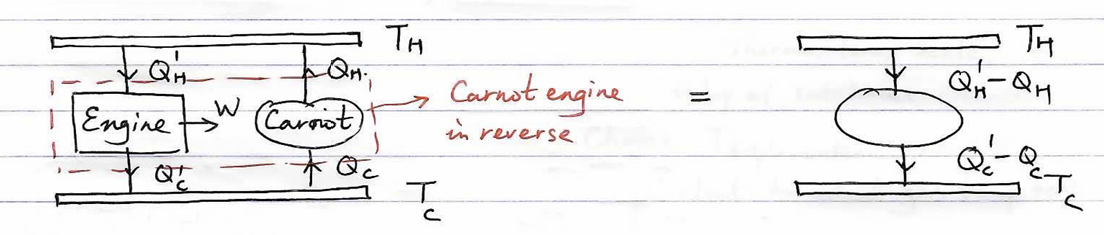
\includegraphics[height=3.0cm]{5.png}
  
  \caption{come from ZCYang}
  
  
  \end{figure}

为了保证第二定律成立,必然要有$Q_H^\prime+Q_H\geq0$\footnote{请注意,这里和图上标定不同,是因为本笔记采用如下的约定:无论文字描述如何,一旦使用$Q$这个符号,一律表示系统在某处吸收的热量,因此所有的系统放热的多少均表示为$-Q$。}。因此,我们得到式(2.22):
\begin{equation}
  \eta_A=\frac{W}{Q_H^\prime}\leq-\frac{W}{Q_H}=\eta_B
\end{equation}

卡诺定理得证。同时根据卡诺定理,我们可以知道,单一高温和单一低温之间的所有可逆热机的效率相同,也就是说,单一高低温之间的可逆热机的效率是二元函数。
\begin{equation}
  \eta=\eta(T_1,T_2)
\end{equation}

考虑工作在单一高温$T_1$和单一低温$T_2$之间的可逆热机A,我们可以写出它的效率$\eta_A$;考虑工作在单一高温$T_1$和单一低温$T_3$之间的可逆热机B,我们可以写出它的效率$\eta_B$。我们总是可以找到这样的一组A和B,使得单次循环中,A和B在$T_1$处吸热相等。此时,B和A的逆过程叠加组成了一个新的可逆热机C,工作在单一高温$T_2$和单一低温$T_3$之间。

考虑C的热机效率。由式(2.23)我们可以写出:
\begin{equation}
  \eta_C=\eta_C(T_2,T_3)
\end{equation}

同时我们又有:
\begin{equation}
 1- \eta_C=\frac{Q_3}{Q_2}=\frac{Q_3}{Q_1}\frac{Q_1}{Q_2}=\frac{1-\eta_B}{1-\eta_A}
\end{equation}

请注意,$1-\eta$应该也是一个只与高低温有关的函数,即$1-\eta=f(T_1,T_2)$,因此我们有:

\begin{equation}
  f(T_2,T_3)=\frac{f(T_1,T_3)}{f(T_1,T_2)}
\end{equation}

于是我们可以得到:
\begin{equation}
  f(T_1,T_2)=\frac{g(T_2)}{g(T_1)}
\end{equation}

请注意,$f$是一个可观测量。我们可以随便找个物质来构建可逆热机,通过观察热机效率我们就可以得到$f$。因此,如果我们标定一个标准点(实际上采用的水的三相点),以$g$作为温度函数,我们就可以得到一种完全不依赖于测温物质的温标。我们称之为热力学温标。(理想气体温标仍然依赖于理想气体作为测温物质,总是显得不那么“普适”)



于是工作在单一高温和单一低温之间的热机效率为:
\begin{equation}
  \eta=1-\frac{T_2}{T_1}
\end{equation}
其中$T_1$,$T_2$分别表示高温和低温的温度。



\subsection{克劳修斯不等式与熵}

任何一个可逆过程总是可以通过划分微元划分成无数小的卡诺循环。(卡诺循环指的就是工作在单一高温和单一低温之间的可逆循环)。我们已经知道,对于一个卡诺循环,有:
\begin{equation}
  -\frac{Q_1}{Q_2}=\frac{T_1}{T_2}
\end{equation}

 稍作修改可以写:
\begin{equation}
  \frac{Q_1}{T_1}+\frac{Q_2}{T_2}=0
\end{equation}

这些循环的叠加,可以有:
\begin{equation}
  \sum_{i}\frac{Q_i}{T_i}=0
\end{equation}

微元划分到极限的程度,我们需要用积分的形式来表示,则有:
\begin{equation}
  \oint\frac{\text{\dj}Q}{T}=0
\end{equation}

以上的推导全部基于循环是可逆循环。如果循环是一般的,则(2.29)式应当写为:
\begin{equation}
  1+\frac{Q_1}{Q_2}\leq1-\frac{T_1}{T_2}\end{equation}

因此,(2.29)式中的等号在一般情况下应当写为大于号,(2.30)-(2.32)中的等号在一般情况下应该改写为小于号。因此我们就有,一般情况下的克劳修斯不等式(2.34),当循环可逆时,克劳修斯不等式取等。\footnote{请注意,当循环不可逆时,可能存在一些非平衡态,这时候我们无法定义温度。因此这里的温度实际上指的是热源在输送热量时的温度。}
\begin{equation}
  \oint \frac{\text{\dj}Q}{T}\leq0
\end{equation}

注意到对于可逆循环,回路积分取零。回路积分取零总是意味着存在某种状态量(例如经典的,电场的环路积分为零),这里采用相似的思路,我们可以得到:
\begin{equation}
  \int_{i(w_1)}^f\frac{\text{\dj}Q}{T}=\int_{i(w_2)}^f\frac{\text{\dj}Q}{T}
\end{equation}

其中$w_1$和$w_2$表示从状态$i$到状态$f$的两种不同的可逆路径。由此可见,我们可以定义一个表示状态之间差值的量,我们把它称为熵。熵的定义式如下:
\begin{equation}
  \Delta S_{if}=\int_{i(w)}^f\frac{\text{\dj}Q}{T}
\end{equation}

其中,我们要求过程$w$是可逆的。如果路径是不可逆的,我们就有:
\begin{align}
\Delta S_{if}>\int_i^f\frac{\text{\dj}Q}{T}\\
\text{\dj}Q<T\mathrm{d}S
\end{align}

到这个时候,热力学第一定律的微分形式终于可以完全依靠状态量来表出:

\begin{equation}
\mathrm{d}U=T\mathrm{d}S-p\mathrm{d}V
\end{equation}

很多时候,粒子数的变化要求被考虑。考虑粒子数变化时,第一定律将改写为:
\begin{equation}
\mathrm{d}U=T\mathrm{d}S-p\mathrm{d}V+\mu\mathrm{d}N
\end{equation}

其中$\mu$是化学势。因此我们就得到:

\begin{align}
U=U(S,V,N)\\
T=\left(\frac{\partial U}{\partial S}\right)_{V,N}\\
-p=\left(\frac{\partial U}{\partial V}\right)_{S,N}\\
\mu=\left(\frac{\partial U}{\partial N}\right)_{V,S}
\end{align}



\subsection{熵增加原理}
考虑一个绝热过程。如果这个绝热过程是可逆的,显然我们可以得到$\Delta S_{if}=0$,如果该绝热过程是不可逆的,根据(2.38),我们得到$\Delta S_{if}>0$。

从这里我们可以推知,第一,一个孤立系统的熵不会减少;第二,随着原本加诸于一个系统的约束被释放,系统会朝着熵增加或至少熵不变的方向移动。至于熵是否真的增加,要取决于过程是否可逆。

\noindent 例1:理想气体的绝热自由膨胀

\noindent 例2:固体的热传导

\subsection{内能的广延性}
当气体不是理想气体时,$U$的广延性总是应当表现为:
\begin{equation}
U=U_1+U_2+U_{bt}
\end{equation}

其中$U_{bt}$是两部分粒子之间的相互作用能。但是实际操作(即热力学极限下)中,我们总是有 $U_{bt}=0$ 。这有两个条件:
 \begin{itemize}
  \item 体系处于热力学极限下($N$无穷);很显然,当体系中个体的数量较少时,即使粒子数密度保持和无穷多粒子体系的数密度相同,体系间的相互作用能也是不可忽略的。因此趋于无穷的粒子数密度是必要的。
\item 内能表示的相互作用是短程相互作用。$U_1$和$U_2$显然是正比于体系的体积的。但$U_{bt}$显然是正比于接触面积(只有当相互作用是短程相互作用的时候才成立)。也正因此,我们可以放心地忽略体系间的相互作用能。
 \end{itemize}

数学上,$U$的广延性可以表示为:
\begin{equation}
  U(\lambda S,\lambda N,\lambda V)=\lambda U(S,N,V)
\end{equation}

 也就是说,$U$是$S,N,V$的齐次函数。两侧同时对$\lambda$求导并代入$\lambda=1$,我们就得到:
 \begin{equation}
  \frac{\partial U}{\partial S}S+\frac{\partial U}{\partial N}N+\frac{\partial U}{\partial V}V=U
 \end{equation}

因此我们就得到:
\begin{equation}
  U=TS-PV+\mu N
\end{equation}

但是,这时候如果我们再取$U$的微分,我们就得到:
\begin{equation}
  \mathrm{d}U=T\mathrm{d}S+S\mathrm{d}T-P\mathrm{d}V-V\mathrm{d}P+\mu\mathrm{d}N+N\mathrm{d}\mu
\end{equation}

这是从$U$的广延性导出的,为了和前面推导出的内能微分表达式保持统一,我们必须承认有:
\begin{equation}
  S\mathrm{d}T-V\mathrm{d}P+N\mathrm{d}\mu=0
\end{equation}

改写这个方程,我们就得到:
\begin{equation}
  \mu=\frac{V}{N}\mathrm{d}P-\frac{S}{N}\mathrm{d}T\end{equation}

这实际上是说明,三个强度量之间并不是独立的。实际上,如果你足够有逆反心理,在(2.41)式时就会对这种说法提出质疑:为什么内能偏偏以这三个量作为函数变量?实际上,内能函数的变量选取确实不是唯一的(只要是三个独立的变量就可以)。之所以选择$S,V,N$,只是因为一方面,这三个都是广延量,有助于我们后面的推导;另外,这三个都作为微分出现在了内能微分的表达式中,方便我们自然地推导出下面的偏导关系。

不过,经过内能广延性的讨论,我们已经知道,至少$P,T,\mu$三个强度量不是相互独立的。

从物理的角度,这实际上也是合理的。因为我完全可以在保证强度量不变的前提下,多加一些气体,这时候内能显然会跟着改变。也就是说,要得到一个作为广延量的内能的值,我们至少要知道一个广延量作为“数量”的量度。
\section{ 其它热力学函数}
与内能类似地,我们还可以定义以下几种热力学函数\footnote{有关这里,可以用附录$A$辅助理解。}:
\begin{align}
  F(T,V,N)=U-TS\\
  \mathrm{d}F=-S\mathrm{d}T-p\mathrm{d}V+\mu\mathrm{d}N\\
  H(S,p,N)=U+PV\\
  \mathrm{d}H=T\mathrm{d}S+V\mathrm{d}p+\mu\mathrm{d}N\\
  G(T,p,N)=U-TS+PV\\
  \mathrm{d}G=-S\mathrm{d}T+V\mathrm{d}p+\mu\mathrm{d}N
\end{align}

某些情况下,我们可以用这些热力学函数来表征不可逆过程的方向。例如,$T,p$固定的情况下,我们有:

\begin{equation}
  \mathrm{d}G=\text{\dj}Q-T\mathrm{d}S\leq0
\end{equation}

又例如,$T,V$固定的情况下,我们有:
\begin{equation}
  \mathrm{d}F=\text{\dj}Q-T\mathrm{d}S\leq0\end{equation}

同时,很显然$G$满足方程:
\begin{equation}
  G(T,p,\lambda N)=\lambda G
\end{equation}

两侧分别对$\lambda$求导并取$\lambda=1$,我们可以得到$G=\mu N$,这也符合前面我们得到的$U$的公式。
\subsection{响应函数}
响应函数一般都是一些方便实验观测的量,其存在意义是为了验证热力学理论的正确性。常用的响应函数有以下几个:
\begin{align}
  \alpha=\frac{1}{V}\left(\frac{\partial V}{\partial T}\right)_p\\
\beta=\frac{1}{p}\left(\frac{\partial p}{\partial T}\right)_v\\
\kappa_T=-\frac{1}{V}\left(\frac{\partial V}{\partial p}\right)_T
\end{align}

应用关系:$\left(\frac{\partial a}{\partial b}\right)_c\left(\frac{\partial b}{\partial c}\right)_a\left(\frac{\partial c}{\partial a}\right)_b=-1$,可以得到:

\begin{equation}
p\beta \kappa_T=\alpha
\end{equation}

\section{麦克斯韦关系}
麦克斯韦关系就是上面四个热力学函数交换求偏导顺序得到的结果,因此一般有四个常见的麦克斯韦关系:

\begin{align}
\left(\frac{\partial S}{\partial V}\right)_T=\left(\frac{\partial p}{\partial T}\right)_v\\
\left(\frac{\partial T}{\partial p}\right)_S=\left(\frac{\partial V}{\partial S}\right)_p\\
\left(\frac{\partial T}{\partial V}\right)_S+\left(\frac{\partial p}{\partial S}\right)_v=0\\
\left(\frac{\partial S}{\partial p}\right)_T+\left(\frac{\partial V}{\partial T}\right)_p=0
\end{align}


\subsection{应用响应函数和麦克斯韦关系的一个例子}

\begin{align}
  C_p-C_v&=T\left(\left(\frac{\partial S}{\partial T}\right)_p-\left(\frac{\partial S}{\partial T}\right)_v\right)\\
  &=T\left(\left(\frac{\partial S}{\partial T}\right)_v+\left(\frac{\partial S}{\partial V}\right)_T\left(\frac{\partial V}{\partial T}\right)_p-\left(\frac{\partial S}{\partial T}\right)_v\right)\\
&=T\left(\frac{\partial S}{\partial V}\right)_T\left(\frac{\partial V}{\partial T}\right)_p\\
&=T\left(\frac{\partial p}{\partial T}\right)_v\left(\frac{\partial V}{\partial T}\right)_p\\
&=TpV\beta\alpha
\end{align}

\section{热平衡的再讨论}
一个孤立系统在平衡时熵要取极大值。因此,如果我们把一个孤立系统分为两部分,则应该有:
\begin{equation}
  S(U,V,N)=S_1+S_2
\end{equation}

系统处于平衡状态时,应该有:
\begin{equation}
  0=\delta S=\delta S_1+\delta S_2=\frac{\partial S_1}{\partial U_1}\delta U_1+\frac{\partial S_1}{\partial V_1}\delta V_1+\frac{\partial S_1}{\partial N_1}\delta N_1+\frac{\partial S_2}{\partial U_2}\delta U_2+\frac{\partial S_2}{\partial V_2}\delta V_2+\frac{\partial S_2}{\partial N_2}\delta N_2
\end{equation}

对于孤立系统,我们又有:
\begin{align}
  \delta U_1+\delta U_2=0\\
  \delta S_1+\delta S_2=0\\
  \delta N_1+\delta N_2=0
\end{align}

代入原式,我们就得到:

\begin{equation}
  0=\delta S=\left(\frac{\partial S_1}{\partial U_1}-\frac{\partial S_2}{\partial U_2}\right)\delta U_1+\left(\frac{\partial S_1}{\partial V_1}-\frac{\partial S_2}{\partial N_2}\right)\delta V_1+\left(\frac{\partial S_1}{\partial N_1}-\frac{\partial S_2}{\partial N_2}\right)\delta N_1
\end{equation}

通过内能的微分表达式,我们又可以得到:
\begin{equation}
  \mathrm{d}S=\frac{\mathrm{d}U}{T}+\frac{p\mathrm{d}V}{T}-\frac{\mu \mathrm{d}N}{T}
\end{equation}

于是我们就得到,处于平衡条件时,体系处处的$T,p,\mu$都保持一致。

此时,我们已经完成了$S$为极值情况下的计算。但是,如前所述,$S$在此时将会取到极大值,因此我们还需要使用极“大”值条件,也就是稳定条件,这是一个二阶条件:
\begin{align}
\delta^2 S&=\sum_{i=1}^2\left(\delta\left(\frac{\partial S_i}{\partial U_i}\right)\delta U_i+\delta\left(\frac{\partial S_i}{\partial V_i}\right)\delta V_i+\delta\left(\frac{\partial S_i}{\partial N_i}\right)\delta N_1\right)\\
&=\sum_{i=1}^2\left(\delta\left(\frac{1}{T_i}\right)\delta U_i+\delta\left(\frac{p_i}{T_i}\right)\delta V_i+\delta\left(\frac{-\mu_i}{T_i}\right)\delta N_i\right)\leq0
\end{align}

这里,考虑$1,2$两个子系统有着相反的变化,它们对系统总的二阶微分差值一定是同向的,也就是说,上面这个式子可以写成更普遍的:

\begin{align}
 & \delta\left(\frac{1}{T}\right)\delta U+\delta\left(\frac{p}{T}\right)\delta V+\delta\left(\frac{-\mu}{T}\right)\delta N\\
  &=-\frac{\delta T}{T^2}\delta U+\frac{T\delta p-p\delta T}{T^2}\delta V-\frac{T\delta\mu-\mu\delta T}{T^2}\delta N\\
  &=-\frac{\delta U+p\delta V-\mu\delta N}{T^2}\delta T+\frac{\delta p\delta V}{T}-\frac{\delta\mu\delta N}{T}\\
  &=\frac{-\delta S\delta T+\delta p\delta V-\delta\mu\delta N}{T}\leq0
\end{align}

最终我们就得到二阶条件:\footnote{请注意这里面只有三个独立变量。而且,与前面不同,在这个方程里你可以任选三个作为独立变量组。}
\begin{equation}
  -\delta S\delta T+\delta p\delta V-\delta\mu\delta N\leq0
\end{equation}

我们可以针对这个式子给一个例子。为了简单起见,我们考虑$N$固定的体系。也就是说,此时体系的独立变量降为两个,我们不妨取为$T,V$。那么,此时我们就应该有:
\begin{align}
  S=S(V,T)\\
  p=p(V,T)\end{align}

  带回到前面得到的式子,我们就能得到:
  \begin{align}
    &-\left(\left(\frac{\partial S}{\partial V}\right)_T\delta V+\left(\frac{\partial S}{\partial T}\right)_v\delta T\right)\delta T+\left(\left(\frac{\partial p}{\partial V}\right)_T\delta V+\left(\frac{\partial p}{\partial T}\right)_v\delta T\right)\delta V\\
    &=-\frac{C_v}{T}(\delta T)^2+\left(\frac{\partial p}{\partial V}\right)_T(\delta V)^2\leq0
  \end{align}  

 为了使得上面这个不等式成立,我们就得到了:
 \begin{align}
  C_v\geq0\\
  \kappa_T\geq0
 \end{align}

这就是平衡的二阶条件。


















\section{气-液相变}
对于相变来说,相图是十分重要的概念。相图给出了在给定参数的情况下体系的相态。相图常用$p,T$作为参数。(插图)

\begin{figure}[h]
  \centering 
  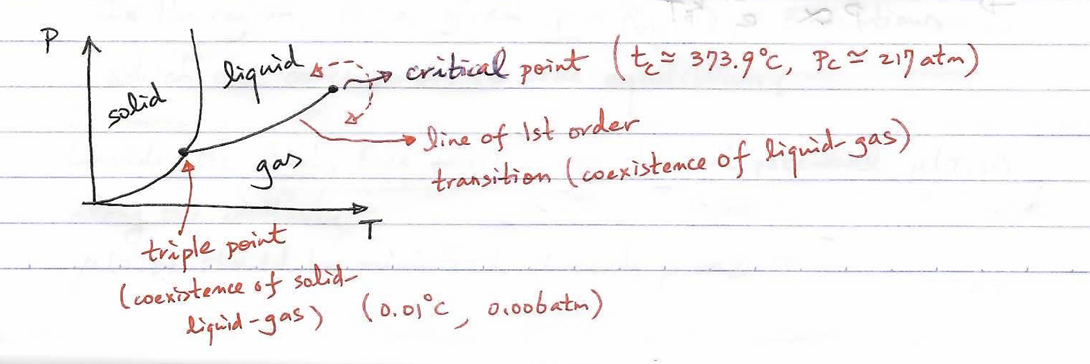
\includegraphics[height=5.0cm]{6.png}
  \caption{come from ZCYang}
\end{figure}

需要指出的是,相图上的边界曲线都代表了一级相变,而在气液相变曲线的右侧(这条线终结于临界点),会存在一个区域,对应二级相变。一级相变是间断的,很容易就能区分不同的相态;但二级相变是连续相变,不会存在从一个相到另一个完全不同的相的跃迁。或者,我们可以从$p-V$图上的等温线来理解。

\begin{figure}[ht]
  \centering 
  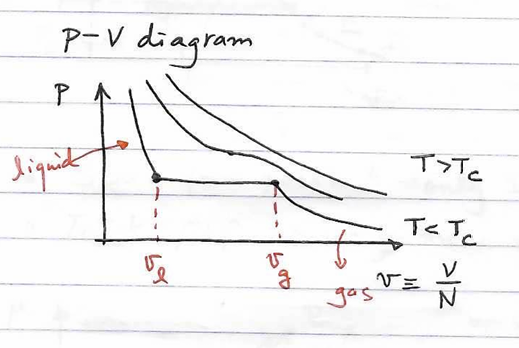
\includegraphics[height=5.0cm]{7.png}
  \caption{come from ZCYang}
\end{figure}

当$T>T_c$时,为二级相变,气体可以近似认为是理想气体,因此其等温线类似理想气体的等温线;当$T<T_c$时,气体开始需要经过两相共存线,因此会存在一段平直的曲线,这段平直曲线就是一级相变的部分。

也因此,临界点就是那个刚好平直段消失的温度。

显然,我们前面得到了一个等式:
\begin{equation}
  \mu=\frac{V}{N}\mathrm{d}P-\frac{S}{N}\mathrm{d}T\end{equation}

因此,$V$可以被认为是一阶偏导数$\left(\frac{\partial \mu_n}{\partial p}\right)_T$,因此,$V$的相变被称为一级相变。

所有的相变都可以理解为热力学函数在某些区域的非解析行为。


\subsection{两相共存线}
当物质以气体或液体存在时,它们的化学势不同,应当存在两个函数:
\begin{align}
  \mu_g=\mu_g(p,T)\\
  \mu_l=\mu_l(p,T)
\end{align}

在两相共存线上,应当有:
\begin{equation}
  \mu_g=\mu_l
\end{equation}

这个条件可以给出共存线的方程。如果我们写出这条线的微分形式,也就是:
\begin{align}
  \mathrm{d}\mu_g=-s_g\mathrm{d}T+v_g\mathrm{d}p&=-s_l\mathrm{d}T+v_l\mathrm{d}p=\mathrm{d}\mu_l     \\
  \frac{\mathrm{d}p}{\mathrm{d}T}&=\frac{s_g-s_l}{v_g-v_l}
\end{align}

我们定义相变潜热就是一团物体在不改变温度的情况下单纯地进行相态转变时吸收的热量,即:
\begin{equation}
  L=T(S_2-S_1)
\end{equation}

于是我们就得到克拉珀隆方程:
\begin{equation}
  \frac{\mathrm{d}p}{\mathrm{d}T}=\frac{L}{T\Delta V}
\end{equation}






\newpage
\appendix
\chapter{勒让德变换/Legendre transformation}

\end{document}